%----------------------------------------------------------------------------------------
%    TITLE PAGE
%----------------------------------------------------------------------------------------

\title{Tratamento de Exceções}

\author{Prof. Gabriel Rodrigues Caldas de Aquino}

\institute
{
    gabrielaquino@ic.ufrj.br\\

    Instituto de Computação -
    Universidade Federal do Rio de Janeiro % Your institution for the title page
}
\date{Compilado em: \\ \today} % Date, can be changed to a custom date

%----------------------------------------------------------------------------------------
%    PRESENTATION SLIDES
%----------------------------------------------------------------------------------------


%------------------------------------------------
\section{Tratamento de Exceções}
%------------------------------------------------

\begin{frame}
    % Print the title page as the first slide
    \titlepage
\end{frame}



%------------------------------------------------
\begin{frame}{Erro de Sintaxe Vs. Exceção}
    \begin{block}{Pontos de observação}
        \begin{itemize}
            \item \textbf{Erros de Sintaxe}:
                  \begin{itemize}
                      \item Detectados antes da execução
                      \item Exemplo: esquecer dois-pontos (\texttt{:}) em um \texttt{if}
                      \item Mensagem mostra o local aproximado do erro antes de executar o código
                  \end{itemize}

            \item \textbf{Exceções}:
                  \begin{itemize}
                      \item Ocorrem durante a execução do código
                      \item Representam erros lógicos ou condições inesperadas
                            \begin{itemize}
                                \item Exemplos: divisão por zero, tipo incorreto
                            \end{itemize}
                      \item Mostram tipo da exceção e (ex: \texttt{ZeroDivisionError}) encerram a execução do código
                  \end{itemize}
        \end{itemize}
    \end{block}

\end{frame}
\begin{frame}{Erro de Sintaxe Vs. Exceção}
    \begin{alertblock}{Principais Diferenças}
        \begin{itemize}
            \item \textbf{Erro de Sintaxe}:
                  \begin{itemize}
                      \item Impede a execução do código
                      \item Ou seja o código não roda
                      \item Precisa ser corrigido antes de executar
                  \end{itemize}

            \item \textbf{Exceção}:
                  \begin{itemize}
                      \item Ocorre \textbf{durante} a execução do código
                      \item Pode ser tratada com \texttt{try-except}
                      \item Caso seja tratada, o funcionamento do código pode ser recuperado
                  \end{itemize}
        \end{itemize}
    \end{alertblock}
\end{frame}



\begin{frame}[fragile]{Exemplos de Erros de Sintaxe}

    \begin{exampleblock}{Exemplos de Erros de Sintaxe}
        \begin{itemize}
            \item \textbf{Esquecer os dois-pontos}:
                  \begin{verbatim}
if x > 5   # ERRO: falta ':'
    print("Maior que 5")
            \end{verbatim}

            \item \textbf{Parênteses não fechados}:
                  \begin{verbatim}
print("Olá, mundo"   # ERRO: falta ')'
            \end{verbatim}


        \end{itemize}
    \end{exampleblock}


\end{frame}


\begin{frame}[fragile]{Exemplos de Exceções em Python}

    \begin{exampleblock}{Exemplos Práticos}
        \begin{itemize}
            \item \textbf{ZeroDivisionError}:
                  \begin{verbatim}
10 / 0   # Tenta dividir por zero
            \end{verbatim}

            \item \textbf{NameError}:
                  \begin{verbatim}
print(var_inexistente)  # Variável não definida
            \end{verbatim}

            \item \textbf{TypeError}:
                  \begin{verbatim}
"2" + 2  # Concatenação de tipos incompatíveis
            \end{verbatim}

            \item \textbf{IndexError}:
                  \begin{verbatim}
lista = [1, 2]
lista[3]  # Acesso a índice inexistente
            \end{verbatim}
        \end{itemize}
    \end{exampleblock}


\end{frame}


\begin{frame}{Mas o que é uma exceção?}
    \begin{block}{Definição}
        Uma exceção é um acontecimento inesperado ou incomum no fluxo normal do código.
    \end{block}

    \begin{block}{Características principais}
        \begin{itemize}
            \item Situações que fogem do comportamento esperado do código
                  \begin{itemize}
                      \item Podemos prever ou não
                  \end{itemize}
            \item Códigos podem lançar exceções intencionalmente
            \item \texttt{ZeroDivisionError} e \texttt{ValueError} são exemplos de exceções
        \end{itemize}
    \end{block}

\end{frame}

\begin{frame}{Então, exceção é isso!}
    \begin{block}{Pontos principais}
        \begin{itemize}
            \item \textbf{Interrompem} no fluxo normal do programa
            \item Ocorrem quando algo \textbf{inesperado} acontece
            \item Exemplos:
                  \begin{itemize}
                      \item Tentar abrir um arquivo que não existe
                      \item Dividir um número por zero
                      \item Acessar uma posição inválida em uma lista
                  \end{itemize}
        \end{itemize}
    \end{block}

    \begin{exampleblock}{Por que tratar exceção é importante?}
        \begin{itemize}
            \item Permitem \textbf{recuperar} o programa de erros
            \item Evitam que o programa \textbf{trave} completamente
            \item Oferecem \textbf{feedback} útil para depuração
        \end{itemize}
    \end{exampleblock}


\end{frame}

\begin{frame}{Entendendo as Mensagens de Erro}
    \begin{columns}
        % Coluna esquerda (explicação)
        \begin{column}{0.5\textwidth}
            \begin{alertblock}{Mensagem de Erro}
                \begin{itemize}
                    \item \textcolor{red}{\textbf{Traceback}}:
                          \begin{itemize}
                              \small
                              \item Histórico que levou ao erro
                          \end{itemize}

                    \item \textcolor{red}{\textbf{Localização}}:
                          \begin{itemize}
                              \small
                              \item \texttt{path/to/file.py}
                              \item Linha 3: \texttt{c=a/b}
                          \end{itemize}

                    \item \textcolor{red}{\textbf{Tipo da Exceção}}:
                          \begin{itemize}
                              \small
                              \item Classe do erro
                              \item ex: \texttt{ZeroDivisionError}
                          \end{itemize}

                    \item \textcolor{red}{\textbf{Descrição}}:
                          \begin{itemize}
                              \small
                              \item Explicação legível do problema
                              \item ex: "division by zero"
                          \end{itemize}
                \end{itemize}
            \end{alertblock}


        \end{column}

        % Coluna direita (screenshot)
        \begin{column}{0.5\textwidth}
            \vspace{-0.5cm}
            \begin{figure}
                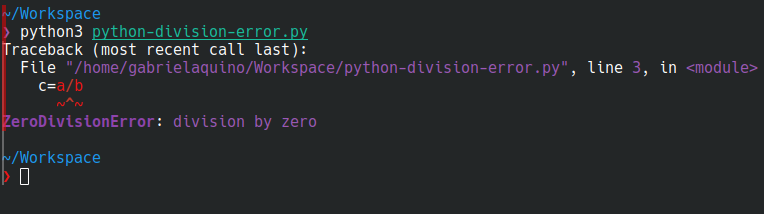
\includegraphics[width=\textwidth]{Images/python-division-error.png}
                \caption{\footnotesize Exemplo de mensagem}
            \end{figure}


        \end{column}
    \end{columns}
\end{frame}


\begin{frame}[fragile]{Try/Except}
    \vspace{-0.3cm}
    \begin{columns}[T]
        % Coluna 1 - Código problemático
        \begin{column}{0.48\textwidth}
            \begin{block}{Código Original}
                \begin{verbatim}
a = 10
b = 0
c = a / b  # Problema aqui
print(c)
            \end{verbatim}


            \end{block}
        \end{column}

        % Coluna 2 - Solução
        \begin{column}{0.48\textwidth}
            \begin{block}{Versão Corrigida com Try/Except}
                \begin{verbatim}
a = 10
b = 0

try:
    c = a / b
except ZeroDivisionError:
    print("Erro: Divisão por zero")
    c = float('inf') # Valor padrão
            \end{verbatim}


            \end{block}
        \end{column}
    \end{columns}

\end{frame}

\begin{frame}{Fluxo de Execução}

    \begin{exampleblock}{Fluxo de Execução}
        \centering
        \begin{tikzpicture}[node distance=1.5cm]
            \node (try) [rounded rectangle, draw, fill=blue!20] {Bloco Try};
            \node (except) [rounded rectangle, draw, fill=red!20, right of=try, xshift=2cm] {Bloco Except};
            \node (sucesso) [below of=try, yshift=-0.7cm] {Execução normal};
            \node (falha) [below of=except, yshift=-0.7cm] {Tratamento do erro};

            \draw [->] (try) -- node[left] {Sem erros} (sucesso);
            \draw [->] (try) -- node[above] {Erro} (except);
            \draw [->] (except) -- (falha);
        \end{tikzpicture}
    \end{exampleblock}

    \begin{alertblock}{Como podemos fazer o tratamento?}
        \begin{itemize}
            \item Especificar o tipo de exceção
            \item Registrar que ocorreu um problema
            \item Definir valores padrão caso tenha um problema
        \end{itemize}
    \end{alertblock}
\end{frame}

\begin{frame}[fragile]{Exemplo  de tratamento}
    \begin{block}{Exemplo de tratamento}
        \begin{verbatim}
try:
    print("Início do bloco try")
    x = 10 / 0  # O problema ocorre aqui
    print("Esta linha NUNCA será executada")
except ZeroDivisionError:
    print("Erro capturado - divisão por zero")
\end{verbatim}
    \end{block}




\end{frame}

\begin{frame}[fragile]{Qual problema temos aqui?}
    \begin{block}{Código Vulnerável}
        \begin{verbatim}
idade = int(input("Digite sua idade: "))
if idade >= 18:
    print("Maior de idade")
else:
    print("Menor de idade")
\end{verbatim}
    \end{block}

    \begin{alertblock}{O que pode dar errado?}
        Porque esse código é vulnerável ?
    \end{alertblock}


\end{frame}

\begin{frame}[fragile]{Problema com Entrada do Usuário}
    \begin{block}{Código Vulnerável}
        \begin{verbatim}
idade = int(input("Digite sua idade: "))
if idade >= 18:
    print("Maior de idade")
else:
    print("Menor de idade")
\end{verbatim}
    \end{block}

    \begin{alertblock}{O que pode dar errado?}
        \begin{itemize}
            \item \textcolor{red}{ValueError}: Se usuário digitar "dez" em vez de 10
        \end{itemize}
    \end{alertblock}


\end{frame}

\begin{frame}[fragile]{Solução com Tratamento de Exceções}
    \begin{block}{Código com o tratamento de exceção}
        \begin{verbatim}
try:
    idade = int(input("Digite sua idade: "))
    if idade >= 18:
        print("Maior de idade")
    else:
        print("Menor de idade")
except ValueError:
    print("Por favor, digite apenas números!")
\end{verbatim}
    \end{block}




\end{frame}

\begin{frame}[fragile]{O que pode dar errado neste codigo?}
    \begin{block}{Discutam o código abaixo}
        \begin{verbatim}

num = int(input("Número: "))  
print(f"Resultado: {100 / num}")        

\end{verbatim}
    \end{block}

\end{frame}

\begin{frame}[fragile]{Riscos levantados}
    \begin{block}{Pontos de risco}
        \begin{verbatim}
num = int(input("Número: "))            # Risco 1: Valor não inteiro
print(f"Resultado: {100 / num}")        # Risco 2: Divisão por zero
\end{verbatim}
    \end{block}

    \begin{itemize}
        \item \textcolor{red}{ValueError}:
              \begin{itemize}
                  \item Entradas como "vinte", "a"...
              \end{itemize}

        \item \textcolor{red}{ZeroDivisionError}:
              \begin{itemize}
                  \item Divisão por zero caso num=0
              \end{itemize}
    \end{itemize}
\end{frame}

\begin{frame}[fragile]{Solução de Tratamento}
    \begin{block}{Código com Tratamento de Erros}
        \begin{verbatim}
try:
    num = int(input("Número: "))
    print(f"Resultado: {100 / num}")
except ValueError:
    print("Digite um número inteiro válido!")
except ZeroDivisionError:
    print("Não pode ser zero!")
\end{verbatim}
    \end{block}



    \begin{exampleblock}{Exemplo de Execuções}
        \begin{itemize}
            \item Entrada "10" → Resultado: 10.0
            \item Entrada "0" → "Não pode ser zero!"
            \item Entrada "abc" → "Digite um número inteiro válido!"
        \end{itemize}
    \end{exampleblock}
\end{frame}

\begin{frame}[fragile]{O Bloco \texttt{else} no Tratamento de Exceções}
    \begin{block}{Quando usar?}
        O bloco \texttt{else} executa \textbf{somente se}:
        \begin{itemize}
            \item O bloco \texttt{try} for concluído \textbf{sem erros}
            \item Nenhuma exceção foi levantada
        \end{itemize}
    \end{block}

    \begin{block}{Diferença entre fluxos}
        \begin{verbatim}
try:
    # Código que pode falhar
except MinhaExcecao:
    # Executa SE ocorrer erro
else:
    # Executa SE NÃO ocorrer erro
finally:
    # Executa SEMPRE
\end{verbatim}
    \end{block}


\end{frame}



\begin{frame}{O bloco \texttt{finally}}
    \begin{block}{Características do \texttt{finally}}
        \begin{itemize}
            \item \textcolor{blue}{Sempre executa}, independentemente:
                  \begin{itemize}
                      \item Se ocorrer erro \textbf{ou não}
                      \item Se o erro foi tratado \textbf{ou não}
                      \item Se houve \texttt{return} no bloco
                  \end{itemize}

            \item Uso típico para:
                  \begin{itemize}
                      \item Liberar recursos (arquivos, conexões)
                      \item Fazer limpeza
                      \item Registrar/logging de operações
                  \end{itemize}
        \end{itemize}
    \end{block}


\end{frame}


\begin{frame}[fragile]{Fluxo Try-Except-Finally}
    \begin{exampleblock}{Fluxo de Execução com Tratamento de Exceções com o finally}
        \centering
        \begin{tikzpicture}[
                every node/.style={
                        rounded rectangle,
                        draw,
                        minimum width=2.5cm,
                        minimum height=0.8cm,
                        align=center,
                        font=\small,
                        fill=white
                    },
                thick
            ]

            % Nós principais posicionados manualmente
            \node (try) at (0, 0) {Try};
            \node (except) at (4.5, 0) {Except};
            \node (sucesso) at (0, -2) {Código OK};
            \node (erro) at (4.5, -2) {Tratamento};
            \node (finally) at (2.25, -4) {Finally};

            % Setas com rótulos sem borda/preenchimento
            \draw[->] (try) -- node[midway, left, draw=none, fill=none, font=\small] {Sem erros} (sucesso);
            \draw[->] (try) -- node[midway, above, draw=none, fill=none, font=\small] {Erro} (except);
            \draw[->] (sucesso) -- (finally);
            \draw[->] (except) -- (erro);
            \draw[->] (erro) -- (finally);

        \end{tikzpicture}
    \end{exampleblock}
\end{frame}

\begin{frame}[fragile]{O Bloco \texttt{finally} em Python}
    \begin{block}{Funcionamento Básico}
        \begin{verbatim}
arquivo = None
try:
    arquivo = open("dados2.txt", "r")
    # Operações com o arquivo
except FileNotFoundError:
    print("Arquivo não encontrado!")
finally:
    print("Sempre executa")
    if arquivo != None:
        arquivo.close()  # Garante o fechamento
    else:
        print(arquivo)
\end{verbatim}
    \end{block}

\end{frame}

\begin{frame}{Hierarquia de Exceções em Python}
    \begin{block}{}
        \small
        Todas as exceções herdam de \texttt{BaseException}. Veja "Exception hierarchy" em \url{https://docs.python.org/3/library/exceptions.html}
    \end{block}

    \begin{center}
        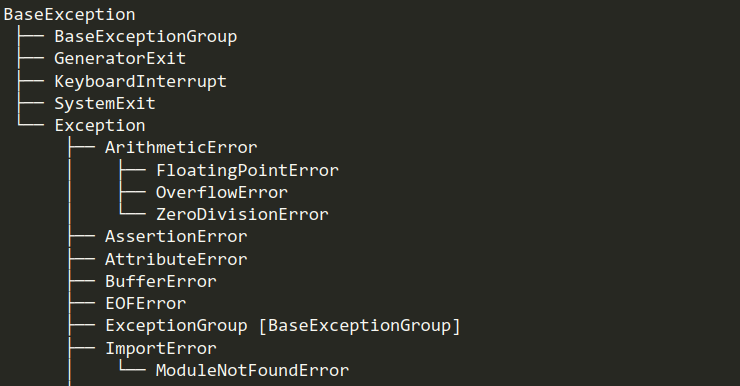
\includegraphics[width=0.8\textwidth]{Images/python_exception_hierarchy.png}
    \end{center}


\end{frame}


\begin{frame}[fragile]{Capturando Exceções Genéricas}
    \begin{block}{Exemplo Prático}
        \begin{verbatim}
try:
    num = int(input("Digite um número: "))
    resultado = 100 / num
    print(f"Resultado: {resultado}")
    
except Exception as err:  
    print(f"Ocorreu um erro: {type(err).__name__}")
    print(f"Mensagem: {str(err)}")
    print(f"Detalhes completo: {err}")
\end{verbatim}
    \end{block}
\end{frame}

\begin{frame}[fragile]{Tratando Diferentes Tipos de Exceções}
    \begin{block}{Exemplo Completo}
        \begin{verbatim}
try:
    num = int(input("Digite um número (não zero): "))
    resultado = 100 / num
    print(f"Resultado: {resultado:.2f}")

except ZeroDivisionError:
    print("Erro: Não é possível dividir por zero!")
except ValueError:
    print("Erro: Digite apenas números inteiros!")

except BaseException as err:
    print()
    print(f"Ops! {type(err).__name__}")
    print(f"Fim!")
\end{verbatim}
    \end{block}

\end{frame}

\begin{frame}[fragile]{Exceções Personalizadas}
    \begin{block}{Como criar uma exceção básica}
        \begin{verbatim}
class MeuErroCustomizado(Exception):
    pass

raise MeuErroCustomizado("Mensagem de erro especial")
\end{verbatim}
    \end{block}

    \begin{exampleblock}{Exemplo Prático}
        \begin{verbatim}
try:
    raise MeuErroCustomizado("Algo deu errado!")
except MeuErroCustomizado as erro:
    print(f"Erro capturado: {erro}")
\end{verbatim}

        \small
        \textbf{Saída:}\\
        \ttfamily
        Erro capturado: Algo deu errado!
    \end{exampleblock}

\end{frame}



\begin{frame}[fragile]{Verificação de Triângulo Equilátero}
    \begin{block}{Código que verifica se os lados formam um triângulo equilátero}
        \begin{verbatim}
def verifica_equilatero(triangulo):
    if triangulo[0] == triangulo[1] == triangulo[2]:
        return True
    else:
        raise ValueError("Não é um triângulo equilátero!")

try:
    lados = [5, 5, 5]  
    if verifica_equilatero(lados):
        print("É um triângulo equilátero!")
except ValueError as e:
    print(f"Erro: {e}")
\end{verbatim}
    \end{block}
\end{frame}

\begin{frame}[fragile]{Exceções - Criando exceções personalizadas}

    \begin{block}{Quando usar?}
        Usada quando precisamos definir nossos próprios tipos de erro para tornar o código mais legível e facilitar o tratamento de erros específicos.
    \end{block}

    \begin{block}{Passo a passo para criação}
        \begin{enumerate}
            \item Criar uma classe que herda de \texttt{Exception}
            \item Definir um construtor (\texttt{\_\_init\_\_}) para personalizar a exceção
            \item Levantar a exceção (\texttt{raise}) no código
            \item Capturar a exceção (\texttt{except}) e tratá-la
        \end{enumerate}
    \end{block}


\end{frame}


\begin{frame}[fragile]{Exceções - Criando exceções personalizadas}

    \begin{block}{1. Criar uma classe que herda de Exception}
        Cada exceção personalizada deve ser uma classe que herda da classe Exception. Isso garante que ela tenha o comportamento de uma exceção normal.
    \end{block}

    \begin{exampleblock}{Exemplo Básico}
        \begin{verbatim}
class SaldoInsuficienteError(Exception):
    """Exceção para indicar que o saldo da conta é insuficiente."""
    pass
\end{verbatim}
    \end{exampleblock}

    \begin{block}{}
        \small
        \texttt{SaldoInsuficienteError} já funciona como uma exceção, mas ainda não tem uma mensagem personalizada.
    \end{block}


\end{frame}

\begin{frame}[fragile]{Exceções - Criando exceções personalizadas}

    \begin{block}{2. Definir um construtor (\texttt{\_\_init\_\_}) para personalizar a exceção}
        Podemos adicionar um construtor para aceitar parâmetros e definir uma mensagem de erro.
    \end{block}

    \begin{exampleblock}{Exemplo com construtor personalizado}
        \begin{verbatim}
class SaldoInsuficienteError(Exception):
    """Exceção para saldo insuficiente."""
    def __init__(self, saldo, valor, 
                 mensagem="Saldo insuficiente para a operação."):
        self.saldo = saldo
        self.valor = valor
        self.mensagem = f"{mensagem} Saldo atual: R${saldo:.2f}, valor 
solicitado: R${valor:.2f}."
        super().__init__(self.mensagem)
\end{verbatim}
    \end{exampleblock}


\end{frame}

\begin{frame}[fragile]{Exceções - Criando exceções personalizadas}

    \begin{block}{3. Levantar a exceção (\texttt{raise}) no código}
        Agora podemos usar \texttt{raise} para lançar essa exceção em uma função.
    \end{block}

    \begin{exampleblock}{Exemplo de uso com \texttt{raise}}
        \begin{verbatim}
def sacar(saldo, valor):
    if valor > saldo:
        raise SaldoInsuficienteError(saldo, valor)
    saldo -= valor
    return saldo
\end{verbatim}
    \end{exampleblock}

\end{frame}


\begin{frame}[fragile]{Exceções - Criando exceções personalizadas}

    \begin{block}{4. Capturar a exceção (\texttt{except}) e tratá-la no código}
        Como qualquer outra exceção, podemos capturá-la com \texttt{try-except}
    \end{block}

    \begin{exampleblock}{Exemplo completo de tratamento}
        \begin{verbatim}
try:
    saldo_atual = 100.0
    novo_saldo = sacar(saldo_atual, 200.0)
    print(f"Saque realizado! Novo saldo: R${novo_saldo:.2f}")
except SaldoInsuficienteError as e:
    print(f"Erro: {e}")
\end{verbatim}
    \end{exampleblock}


\end{frame}

\begin{frame}[fragile]{Criando Exceções Personalizadas}
    \small
    \begin{verbatim}
class SaldoInsuficienteError(Exception):
    def __init__(self, saldo, valor, mensagem="Saldo insuficiente para a 
    operação."):
        self.saldo = saldo
        self.valor = valor
        self.mensagem = f"{mensagem} Saldo atual: R${saldo:.2f}, 
        valor solicitado: R${valor:.2f}."
        super().__init__(self.mensagem)
def sacar(saldo, valor):
    if valor > saldo:
        raise SaldoInsuficienteError(saldo, valor)
    saldo -= valor
    return saldo
try:
    saldo_atual = 100.0
    novo_saldo = sacar(saldo_atual, 20.0)
    print(f"Saque realizado! Novo saldo: R${novo_saldo:.2f}")
except SaldoInsuficienteError as e:
    print(f"Erro: {e}")

\end{verbatim}

\end{frame}

\begin{frame}{Dicas e melhores práticas}
    \begin{itemize}
        \item Não use \textit{except Exception} de forma genérica.
        \item Não use \textit{except} sem nenhuma exceção.
        \item Para pegar uma exceção e tratar, precisa que o código que você queira testar esteja dentro do \textit{try}
        \item Não sabe qual exceção pegar? Leia a documentação do python
              \begin{itemize}
                  \item Google é seu amigo, procure por \textit{"python exception list"}
                  \item ou vá na URL: \url{https://docs.python.org/3/library/exceptions.html}
              \end{itemize}
    \end{itemize}

\end{frame}
